\documentclass[11pt,a4paper,oneside]{article}
\usepackage{graphicx}
\usepackage[usenames,dvipsnames]{xcolor}
\usepackage[section]{placeins}
\usepackage{fancyhdr}
\usepackage{hyperref}
\hypersetup{
    colorlinks,
    citecolor=RoyalBlue,
    filecolor=RoyalBlue,
    linkcolor=RoyalBlue,
    urlcolor=RoyalBlue
}
\usepackage[all]{hypcap}
\pagestyle{fancyplain}

\begin{document}
\lhead{Infographics Generator}
\rhead{Project Plan}
\begin{titlepage}



\begin{center}


\includegraphics[width=1\textwidth]{images/sponsor-logo.png}\\[1cm]    

{ \huge \bfseries Infographics Generator}\\[0.4cm]
{ \large \bfseries Project Plan}\\[0.4cm]

Louis Bodnar\\
Peter Chen\\
Lok Cheung\\
Kevin Shreve\\


\vfill

{\large \today}

\end{center}

\end{titlepage}

\tableofcontents
\newpage
\section{Executive Summary}
Over three decades ago, a professor at Wayne State University took on a challenge that Cadillac deemed unsolvable. That professor was Jim Anderson. His computer-generated dot maps gave Cadillac's marketing department a competitive advantage by allowing them to easily visualize dealership locations across the nation. Jim began using the power of computers to analyze these networks of dealerships and started a company that specialized in the planning and management of these networks. Thus, Urban Science was born.\\

Urban Science is now an international company, headquartered in Detroit, Michigan. They assist nearly every original equipment manufacturer (OEM) in over 60 countries. We designed a web application to show OEMs monthly performance data on vehicle sales, lead management, and service for their primary market area. OEMs use this performance data to adjust spending to maximize their market potential. The appeal of our web application is its ease of use, and visual appeal.\\

In today's world, the display of information is an evolving art. Yesterday's solution was clipart and spreadsheets, but that is no longer enough. We require a more engaging approach to delivering a point. The modern solution is an information graphic or infographic. An infographic is a graphical display that quickly conveys data that would otherwise require a lengthy explanation. Modern infographics use clever design schemes and cartoon characters to keep the viewer interested while showing relationships in the data.\\

Our web application uses a brand new flavor of infographic that is designed to update dynamically. It uses information directly from Urban Science to generate graphics that reflect the most up-to-date monthly data. The web application also provides the ability to view previous months to allow OEMs to refrence historical data.\\

\section{Functional Specifications}
The purpose of our infographics generator is to creatively display information on the iPad.  It simplistically conveys performance data to the manager of a dealership or original equipment manufacturer (OEM).  The main page allows users to select an infographic by swiping through a menu.  Each infographic communicates with a database to ensure it is being displayed with the most current data available.  Users have the ability to change the month of the data being displayed by swiping their fingers across the infographic.  They can also tap on any of the data to see a detailed description of the data and a trend chart to show how it has changed over the last six months.\\

\section{Design Specifications}
\subsection{Overview}
The menu interface is based on a Lazy Susan. A user can swipe their finger across the screen to rotate the icons, and touch any one of them to select a category. Selecting an icon will trigger the infographics generator using the category that was selected. The infographics generator then grabs the preloaded data from local storage and displays it as part of an infographic. The user can then select different infographics to display the other information.\\

\subsection{System Architecture}
The infographic application is comprised of two major components: a web application and a database. Safari displays the menu screen. When an infographic is selected, data will be pulled from the database and kept in local storage so it can be used to generate the infographic.\\

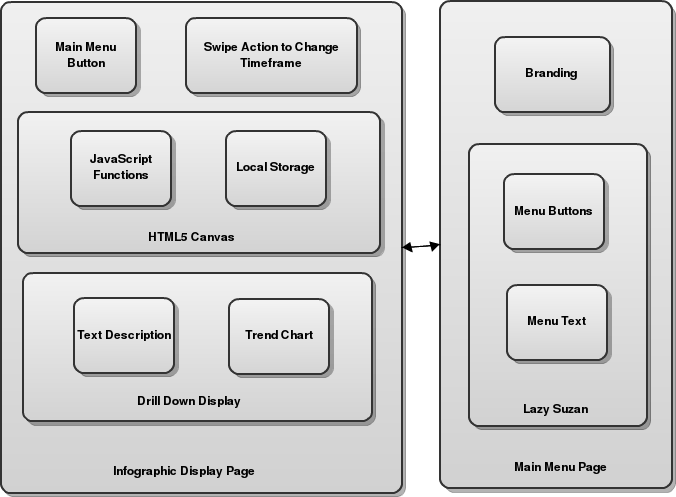
\includegraphics[width=.9\textwidth]{images/Capstone_-_System_Architecture_Diagram.png}\\   
\newpage
\subsection {Main Menu}
This image shows the swiping action that is used to rotate the icons.  Below it is a screenshot of the main menu.  The menu is displayed in a lazy Suzan style to allow the user to scroll through the icons.  The corresponding infographic display page is shown when the icon is clicked.\\

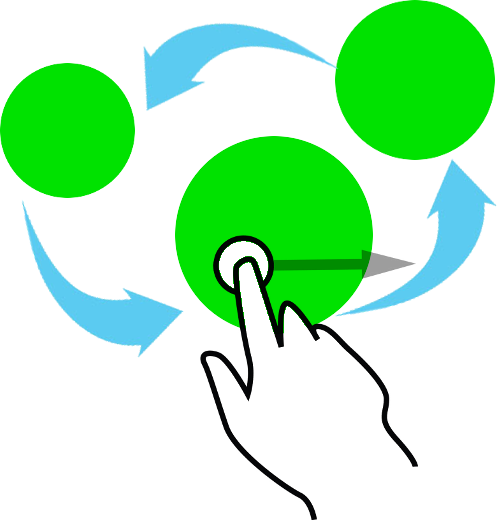
\includegraphics[width=.4\textwidth]{images/switcheroo.png}\\

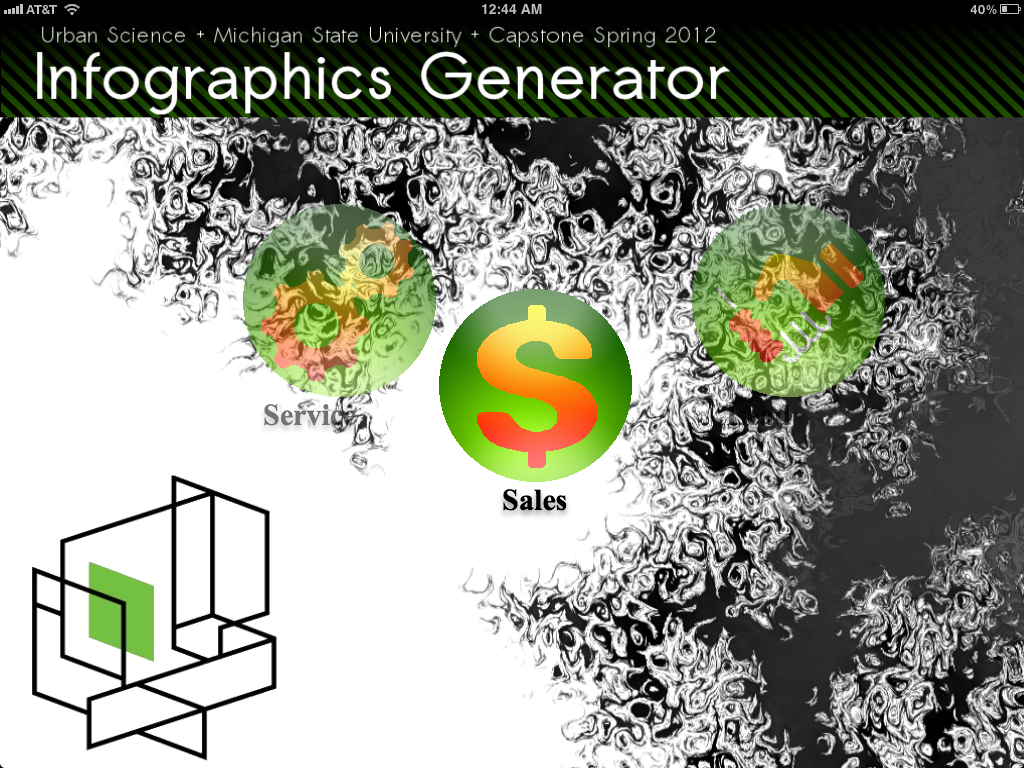
\includegraphics[width=1\textwidth]{images/main-menu.png}\\
\newpage
\subsection{Infographic Page}

This is how the display page looks for the sales infographic.  The current month is displayed at the top right next to the menu button.  The menu button navigates back to the menu screen.  Swiping left and right increases and decreases the month.  Tapping a KPI data brings up additional information.\\

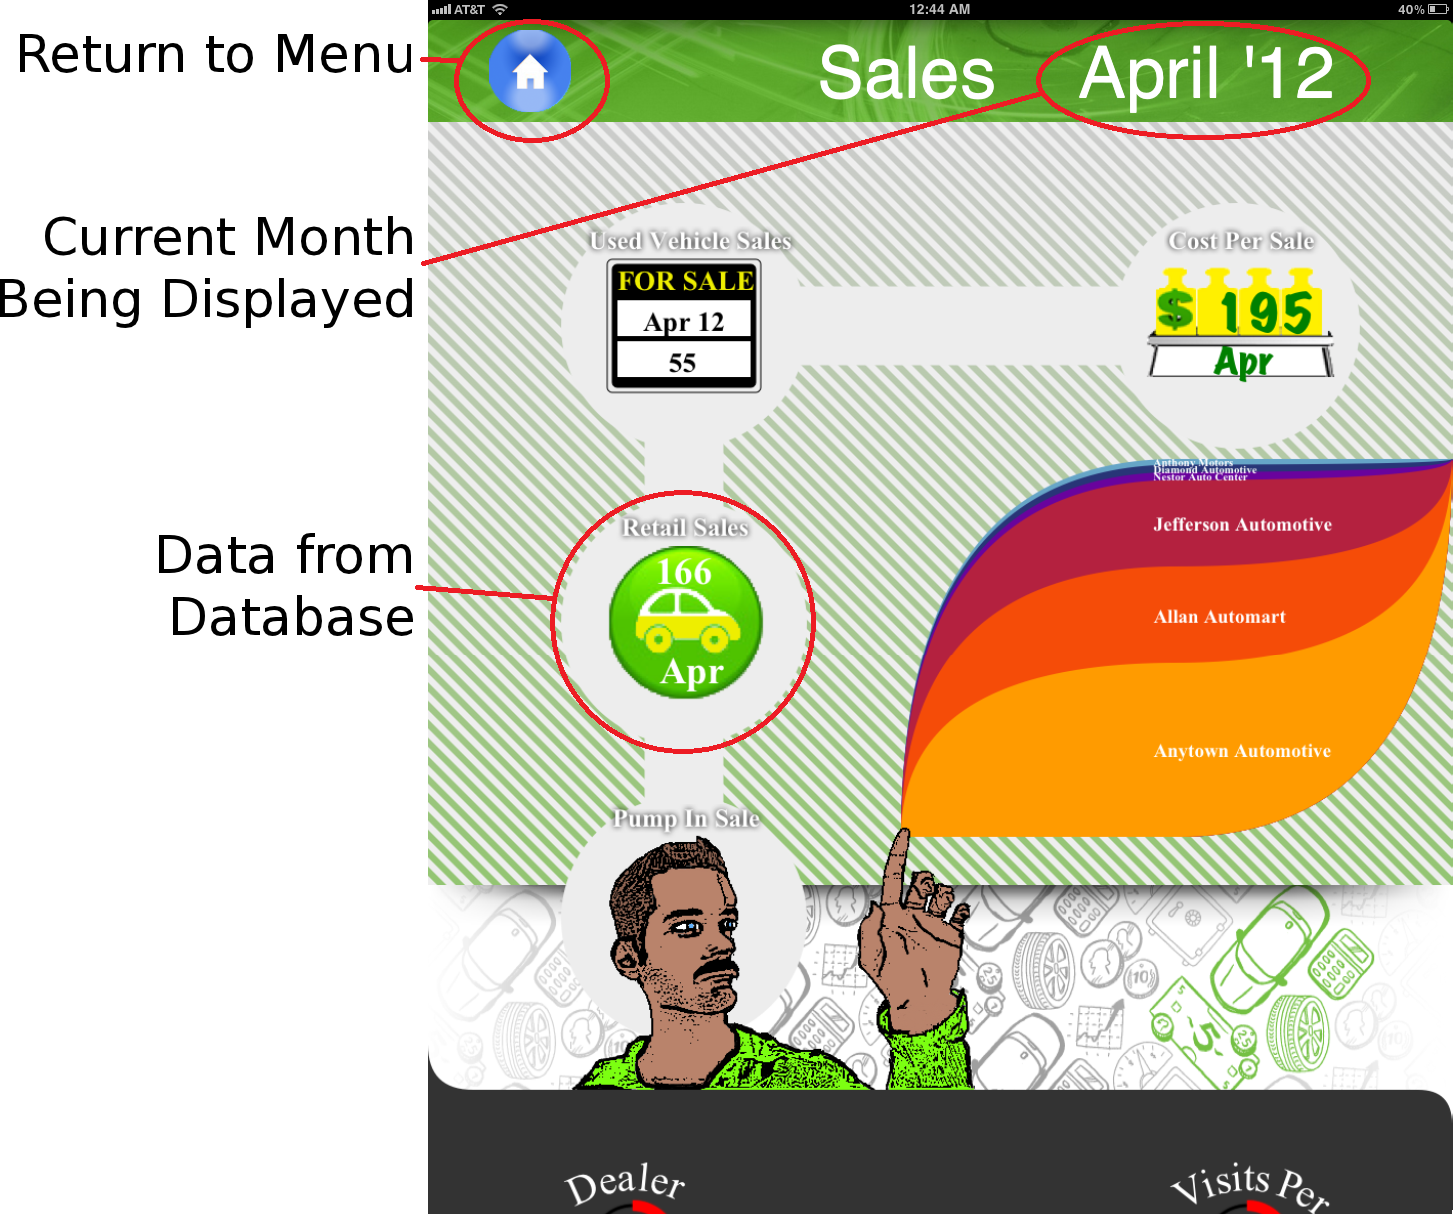
\includegraphics[width=1\textwidth]{images/labels.png}\\

\newpage
\subsection{Drill Down Display}
The drill down display is shown when a KPI data is tapped.  It is a box that appears in the center of the screen with a description of the KPI data and a trend chart which shows the data for the last 6 months.\\

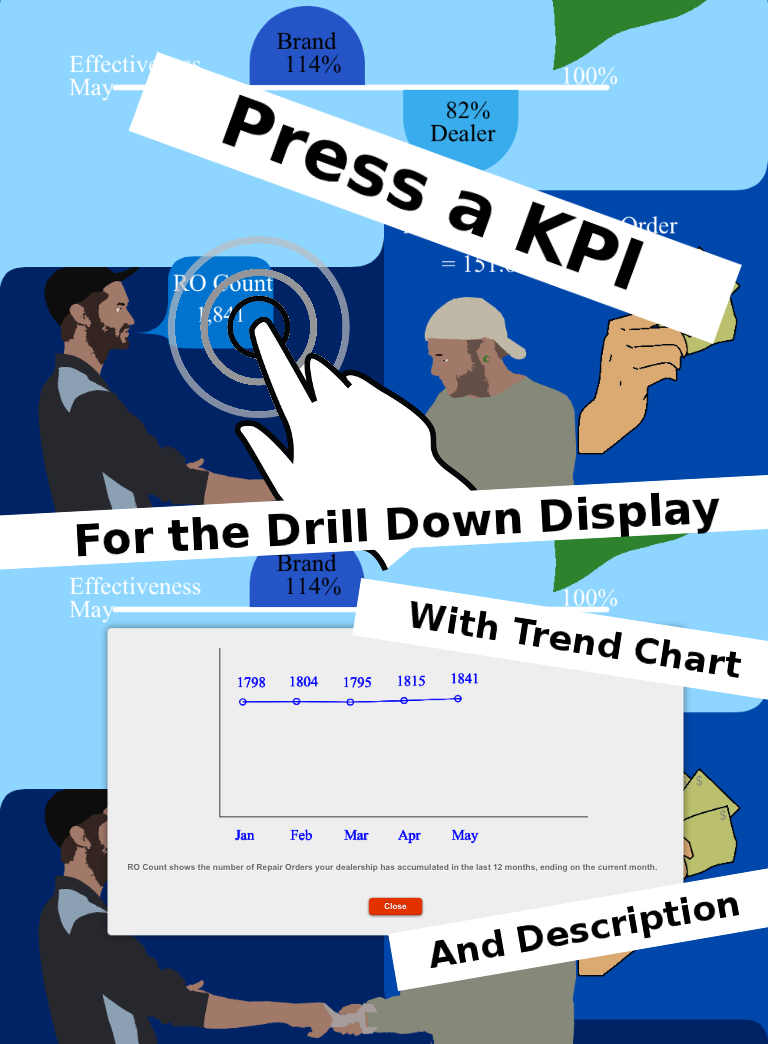
\includegraphics[width=1\textwidth]{images/fun.png}\\
\newpage
\subsection {Web Backend}

The user connects to the web backend via Safari. As the page loads, a script runs to automatically retrieve and store data from the database into temporary local storage. If there is newer data it will update the local storage when the user refreshes the page. This data is used by the infographics generator to update values in the infographic.\\


\section{Technical Specifications}

The infographics generator produces infographics suitable for display on the iPad 2 using the Safari browser.\\

The Index.html page in our webapp contains the infographic selector menu. The infographic selector menu is used to browse all available infographics. The infographics available to choose from include: Sales, Service, and Lead Management. The selector interface has three icons, each representing an infographic, arranged in a horizontally elongated ellipse. A swipe in the left direction causes the icons to rotate clockwise following the elliptical path. Likewise, the icons rotate counter clockwise when swiped in the right direction. By swiping, the user feels that they are causing the invisible lazy suzan to rotate. Upon tapping the front most icon, Safari navigates to the corresponding infographic's page.\\

The infographic display page contains a floating image called the header. The header spans the width of the page and remains at the top of the page when the user scrolls. The header has a button on the left hand side which, if tapping, navigates back to the infographic selector menu. The right side of the header has text displaying the month and year of the data being displayed. The infographic is located immediately beneath the header and spans the entire width of the page. If the infographic is swiped left, the next month's data is displayed. If swiped right, the previous month's data is displayed. If no data exists for the month attempting to be displayed, the current date is not changed.\\

Each infographic displays multiple key performance indicators (KPI) data. The data is obtained from a Microsoft SQL database. The server hosting the infographics generator uses an ASP.NET script (KPI\_Handler.ashx) to query the database for all available KPI data, serializes the data, and returns the data to the client device in JavaScript Object Notation (JSON). The client device then parses this data using a JavaScript function (found in Scripts/KPILocalStorage.js) and adds the data to local storage.\\

An infographic element is a visual representation of KPI data, responsible for displaying one or more KPI data. An infographic is comprised of multiple infographic elements. Each infographic element is drawn on an HTML5 canvas using JavaScript functions found in one of the three infographic drawing files (draw-sales.js, draw-service.js, draw-lead.js) or the common element file (elements.js). The common element file is used to centralize the generic JavaScript functions that are used to draw the elements in the infographics. The infographic specific files call functions from the common element file and have their own JavaScript functions to draw the infographic. They also calls functions to retrieve specific KPI values from local storage.\\

A drill down display is shown in the center of the screen if an infographic element is tapped. The drill down display gives an brief description of the KPI that was tapped and shows a trend chart of the KPI over the last 6 months (ending in the current month) or the maximum number of months available, whichever number is smaller.\\


\section{Schedule}

\subsection{Week 1 (January 9, 2012)}
\begin{itemize}
\item Had our first conference call with our customer
\item Set up weekly conference calls with our customer
\item Set up regular team meetings to meet twice a week
\item Installed virtual machines
\end{itemize}


\subsection{Week 2 (January 16, 2012)}
\begin{itemize}
\item Started UML diagrams
\item Installed Windows Server 2008 R2
\item Installed IIS 7
\item Installed ASP.NET
\item Installed Microsoft SQL Server
\item Talked with our customer about interface mockups
\end{itemize}

\subsection{Week 3 (January 23, 2012)}
\begin{itemize}
\item Completed more UML diagrams
\item First draft of project-plan
\item Installed Visual Studio 2010
\item Created screen mockups
\item Created sample infographic elements
\end{itemize}

\subsection{Milestone: Status Reports}
\begin{itemize}
\item Gave report to class
\end{itemize}

\subsection{Week 4 (January 30, 2012)}
\begin{itemize}
\item Created infographic elements using actual KPI data
\item Wrote website to showcase infographics
\item Decided to work on sales infographic first
\end{itemize}

\subsection{Milestone: Project Plan Presentation}
\begin{itemize}
\item Gave presentation in class
\end{itemize}

\subsection{Week 5 (February 6, 2012)}
\begin{itemize}
\item Presented project plan to class
\item Changed from using XML to JSON for pulling database information
\item Have roundabout working with several images for infographic selector buttons
\item Successfully pulled data from a SQL database using ASP.NET
\end{itemize}

\subsection{Week 6 (February 13, 2012)}
\begin{itemize}
\item Sales infographic exists in basic form
\item Added background image to main menu
\end{itemize}

\subsection{Week 7 (February 20, 2012)}
\begin{itemize}
\item Infographics now use values from database
\item Rewrote pump in sales infographic
\item Practiced Alpha Demonstration
\end{itemize}

\subsection{Milestone: Alpha Demonstrations}
\begin{itemize}
\item Demonstrated software to Urban Science for first time
\item Recieved usefull feedback from Urban Science
\end{itemize}

\subsection{Week 8 (February 27, 2012)}
\begin{itemize}
\item Planning for betas
\item Created mockups of service and lead management infographics
\end{itemize}

\subsection{Week 9 (March 12, 2012)}
\begin{itemize}
\item Added service infographic to website
\item Fixed bugs with swiping
\item Local storage now refreshes with website
\end{itemize}

\subsection{Week 10 (March 19, 2012)}
\begin{itemize}
\item Added MSU and Urban Science branding to website
\item Visited Urban Science headquarters in Detroit, MI
\end{itemize}

\subsection{Week 11 (March 26, 2012)}
\begin{itemize}
\item Added remaining KPI to service and lead management infographics
\item Implemented drill down display
\item Began writing script for video
\item Practiced for Beta presentation
\end{itemize}

\subsection{Milestone: Beta Demonstrations}
\begin{itemize}
\item Presentation was successful
\item Project was feature complete
\end{itemize}

\subsection{Week 12 (April 2, 2012)}
\begin{itemize}
\item Changed text formatting upon customer request
\item Fixed bugs with swiping 
\end{itemize}

\subsection{Week 13 (April 9, 2012)}
\begin{itemize}
\item Updated project plan to reflect most recent version of webapp
\item Discovered origin of grey background in jQuery css file
\item Filmed video
\end{itemize}

\subsection{Week 14 (April 16, 2012)}
\begin{itemize}
\item Edited video
\item Wrote user manual
\item Fixed elevator
\end{itemize}

\subsection{Week 15 (April 23, 2012)}
\begin{itemize}
\item Set up for design day
\item Presented at design day
\end{itemize}

\subsection{Milestone: Projet Video}
\begin{itemize}
\item Filmed using Dr. D's new camera
\item Filmed video in capstone lab
\end{itemize}

\subsection{Milestone: All Deliverables}
\begin{itemize}
\item Successfully submitted
\end{itemize}

\subsection{Milestone: Design Day}
\begin{itemize}
\item Great success!
\end{itemize}




%\section{Remaining tasks}
%\begin{itemize}
%\item clean up code
%\item write documentation for functions
%\item project video
%\item rename /webapp/images/Avg\$.png because of potential problems with having a dollar sign in the filename
%\end{itemize}


\end{document}
